% arara: pdflatex: { synctex: yes }
% arara: makeindex: { style: ctuthesis }
% arara: bibtex

% The class takes all the key=value arguments that \ctusetup does,
% and a couple more: draft and oneside
\documentclass[twoside]{ctuthesis}
\usepackage{algorithmicx}
\usepackage{algpseudocode}
\usepackage{algorithm}
\usepackage{mathtools}

\usepackage{tabularx} % for adjusting table width
\usepackage{caption} % for customizing table caption

\algdef{SE}[DOWHILE]{Do}{doWhile}{\algorithmicdo}[1]{\algorithmicwhile\ #1}%


\ctusetup{
	preprint = \ctuverlog,
%	mainlanguage = english,
%	titlelanguage = czech,
	mainlanguage = english,
	otherlanguages = {slovak,english},
	title-czech = {Moje bakalářka se strašně, ale hrozně dlouhým předlouhým názvem},
	title-english = {My Favourite Thesis; Just the Title is Soooooooo Looooong},
	subtitle-czech = {Cesta do tajů kdovíčeho},
	subtitle-english = {Journey to the who-knows-what wondeland},
	doctype = B,
	faculty = F4,
	department-czech = {Katedra matematiky},
	department-english = {Department of Mathematics},
	author = {Matouš Pelikán},
	supervisor = {Prof. Krutoš Spravedlivý},
	supervisor-address = {Ústav X, \\ Uliční 5, \\ Praha 99},
	supervisor-specialist = {John Doe},
	fieldofstudy-english = {Mathematical Engineering},
	subfieldofstudy-english = {Mathematical Modelling},
	fieldofstudy-czech = {Matematické inženýrství},
	subfieldofstudy-czech = {Matematické modelování},
	keywords-czech = {slovo, klíč},
	keywords-english = {word, key},
	day = 10,
	month = 2,
	year = 2017,
	specification-file = {ctutest-zadani.pdf},
%	front-specification = true,
%	front-list-of-figures = false,
%	front-list-of-tables = false,
%	monochrome = true,
%	layout-short = true,
}

\ctuprocess

\addto\ctucaptionsczech{%
	\def\supervisorname{Vedoucí}%
	\def\subfieldofstudyname{Studijní program}%
}

\ctutemplateset{maketitle twocolumn default}{
	\begin{twocolumnfrontmatterpage}

		\ctutemplate{twocolumn.abstract.in.titlelanguage}
		\ctutemplate{twocolumn.abstract.in.secondlanguage}
		\ctutemplate{twocolumn.tableofcontents}
		\ctutemplate{twocolumn.listoffigures}
	\end{twocolumnfrontmatterpage}
}

% Theorem declarations, this is the reasonable default, anybody can do what they wish.
% If you prefer theorems in italics rather than slanted, use \theoremstyle{plainit}
\theoremstyle{plain}
\newtheorem{theorem}{Theorem}[chapter]
\newtheorem{corollary}[theorem]{Corollary}
\newtheorem{lemma}[theorem]{Lemma}
\newtheorem{proposition}[theorem]{Proposition}

\theoremstyle{definition}
\newtheorem{definition}[theorem]{Definition}
\newtheorem{example}[theorem]{Example}
\newtheorem{conjecture}[theorem]{Conjecture}

\theoremstyle{note}
\newtheorem*{remark*}{Remark}
\newtheorem{remark}[theorem]{Remark}

\setlength{\parskip}{0.5ex plus 0.2ex minus 0.2ex}






% Only for testing purposes
\listfiles
\usepackage[pagewise]{lineno}
\usepackage{lipsum,blindtext}
\usepackage{mathrsfs} % provides \mathscr used in the ridiculous examples

\begin{document}
	
\maketitle


\chapter{Introduction}


Combinatorial optimization problems are a class of challenging tasks that involve finding the best arrangement or combination of discrete elements from a large set of possibilities. These problems arise in various fields, such as logistics, scheduling, network design, and resource allocation. Examples of combinatorial optimization problems include the traveling salesman problem (TSP), the knapsack problem, or the graph coloring problem to name only a few. The complexity of these problems lies in the exponential growth of possible solutions as the problem size increases, making it computationally infeasible to search the entire solution space.

Metaheuristics have emerged as a powerful technique to face the computational challenges posed by complex combinatorial problems. Metaheuristics provide a flexible and robust framework for addressing optimization challenges by operating at a higher level of abstraction. These algorithms offer a unique approach to problem-solving by exploring large solution spaces efficiently and effectively. They are particularly well-suited for combinatorial optimization problems where traditional methods, such as linear programming, integer programming, etc., struggle due to the high-dimensional and non-linear nature of the search space.

Among many other, evolutionary algorithms (EAs) represent a powerful class of metaheuristics that have demonstrated remarkable effectiveness in solving combinatorial optimization problems. Inspired by the principles of natural evolution, these algorithms emulate the process of natural selection and adaptation to guide the search for optimal or near-optimal solutions. They typically work with a population of individuals, where each individual represents a possible solution to the problem at hand. On top of what EAs can offer, it is common practise to integrate local search techniques in order to enhance the performance. Local search focuses on exploring the neighborhood of a given solution to find better nearby solutions. By combining local search with evolutionary algorithms, the search process benefits from both global exploration and local exploitation, leading to improved solution quality and convergence.

An example of such evolutionary based algorithm is IREANN, introduced by Kubalík and Snížek in \cite{kubalik2014novel}. IREANN uses an indirect representation and a so-called nearest neighbor heuristic, which is a constructive procedure suited for routing problems. Both of these concepts used in IREANN are heavily exploited in this thesis. Local search heuristics might be incorporated to IREANN to yield even better performance.

However, given the nature of IREANN's indirect representation functionality, improvements made by local search heuristics would only affect the single individual whose neighborhood of solution space was searched. The information about local improvements can not be easily passed between other individuals in a population. 

The objective of this thesis is to propose an extension to the IREANN algorithm that enables the propagation of valuable information about high-quality features of individual solutions across the entire population during computation. This extension aims to ensure that the entire population can potentially benefit from the insights gained from individually discovered superior features, thereby enhancing the overall performance and optimization capabilities of the algorithm.

The principle of enhancing the algorithm si to incorporate a mechanism that during computation captures and retains information about the features that contibute the most to high-quality solutions. The mechanism involves periodically storing the relevant information which is subsequently used in the nearest neighbor heuristic, and serves as a proxy to information about the actual distance. The whole algorithm was specifically designed to solve the Capacitated arc routing problem (CARP), which is more challenging than the famous TSP and introduces more constraints.

Several slight modifications of above mentioned approach have been implemented as a result of this thesis. The effects of proposed extension on solution quality were empirically verified by testing on standard available CARP benchmark datasets.

The thesis is structured as follows...(TODO)

\chapter{Problem definition}
The capacitated arc routing problem (CARP), firstly introduced by Golden and Wong \cite{golden1981capacitated}, is a subject in combinatorial optimization, commonly appearing in operations research and transportation logistics. In this chapter, we will provide a formal definition of the CARP, establish relevant terminology, and underline the basic properties that characterize this complex problem.

The Capacitated Arc Routing Problem (CARP) is a variant of the arc routing problem where a fleet of vehicles of uniform capacity is used to service a set of arcs or edges in a network. The fundamental challenge is to design the minimum cost set of routes such that each vehicle originates and terminates at a depot, each edge in the network requiring service is traversed by exactly one vehicle, and the total demand serviced by any vehicle does not exceed its capacity.

The problem is defined on a connected, undirected graph \emph{G} = (\emph{V, E}), where V is the set of vertices and E is the set of edges. Every edge \emph{e} $\in$ \emph{E} has a non-negative cost or length \emph{$ c_e $} and a non-negative demand for service \emph{$ d_e $}. The edges with positive demand make up the subset of the required edges \emph{$ E_R $}. In CARP, the graph is typically undirected, meaning that each edge can be traversed in either direction with equal cost. 
The demand \emph{$ d_e $} of an edge \emph{e} represents the quantity of some resource or service that must be delivered along that edge. Each vehicle has a maximum capacity Q and the total demand of all edges in its route cannot exceed this capacity.
Given a vehicle capacity \emph{Q}, the CARP consists
of finding a set of vehicle routes of minimum cost,
such that every required edge is serviced by exactly
one vehicle, each route starts and ends at a prespecified vertex \emph{$ v_0 $} $\in$ \emph{V} (the depot) and the total
demand serviced by a route does not exceed the
vehicle capacity \emph{Q}. The number of maximum vehicles \emph{K} used is also constrained.  Golden and Wong \cite{golden1981capacitated} show that the CARP is NP-hard. 


\chapter{Related work}
Capacitated Arc Routing Problems (CARP) are known to be NP-hard problems. Due to its complexity, it is possible to solve it exactly only for small-sized instances. Instances of larges size usually make use of heuristic, more specifically metaheuristic approaches.

This chapter gives an overview of known 

\section{Exact and lower bound methods}
Lower bound methods provide a tight lower bound on its optimal cost. Such a bound is helpful when evaluating larger CARP instances, where heuristic approach has to be employed, since solving them exactly would be computationally too demanding and not feasible at all. Thus, achieving a solution which is close to a lower bound might be a good measure of quality for heuristic algorithms.
A simplified integer linear model was proposed by Belenguer and Benavent \cite{BELENGUER2003705}. The sparse formulation used does not lead to a valid CARP solutions, but presents very tight lower bounds for the problem. Only one integer is used for each edge, which results in not being able to say which vehicles service which edges.

First possible way of solving CARP is based on transforming the problem into a node routing problem and then using existing VRP methods to solve it. Quality of the solution depends on how well, meaning how compact such a transformation can get. The goal is for the dimension to not increase drastically.
First transformation of its kind was introduced by Pearn, Assad and Golden \cite{PEARN1987285} which reduced the CARP problem into CVRP problem, but was regarded as unpractical, since the transformed CVRP problem had a graph with 3e + 1 vertices, where e is the number of required edges in CARP. Similar transformation was then proposed by Longo, Aragao and Uchoa \cite{LONGO20061823}, which further reduced the number of vertices to 2e + 1. Combined with a branch-and-cut-and-price algorithm, they observed effective results, solving all gdb instances for the first time and finding new optimum for val files and two for egl files.
More recently, a compact transformation was introduced recently by Les Foulds et al. \cite{foulds2015compact} where the number of nodes is at most larger only by one than the number of edges. Again, an adapted version of branch-and-cut-and-price algorithm for CVRPs was used to obtain the results. The authors managed to solve all of the instances from the gdb dataset, however some instances in the larger dataset egl were not solved satisfactorily.

As mentioned by Bode and Irnich \cite{bode2012cut}, converting arc routing problems into node routing ones has significant drawbacks, which are models with inherent symmetry, dense underlying networks or models with huge number of vertices. Therefore, it is worth considering specialized CARP methods to address these issues. 
Specialized exact algorithms for CARP often involve solving integer programs using branch-and-cut or branch-and-bound combined with column generation. Branch-and-cut uses a cutting plane approach, in which inequalities are added to the optimization problem.  By adding these cuts, the feasible region of the subproblems can be further restricted, which can help the algorithm find the optimal solution more efficiently. Column generation, on the other hand, involves iteratively generating and adding columns (variables) to the problem's constraint matrix until an optimal solution is found. Mentioned algorithms are used in \cite{bode2012cut}, \cite{bartolini2013improved} to solve instances with up to 190 nodes to optimality. Instances with number of nodes greater than 200 remain unsolved by exact approaches. 

\section{Heuristics}
Heuristics algorithms are approximate methods that are used to quickly find a solution to an optimization problem that is likely to be close to the optimal solution. They are typically used when the exact optimization problem is too computationally expensive to solve in a reasonable amount of time, which is the case for solving larger instances of the CARP. The main focus will be on meta-heuristics, which represent more general techniques applicable to wide range of optimization problems.

One of the most famous algorithms for solving CARP is a tabu search algorithm called CARPET proposed by Hertz, Laporte and Mitaz \cite{hertz2000tabu}. In CARPET, a solution in represented by a set of nodes representing all traversed edges. Solutions violating vehicle capacity are accepted but penalized. The search process in a tabu search is guided by the tabu rules, which specify which moves are allowed and which are "tabu" (forbidden) at each step. Number of improvement procedures which are used in the search process are presented in CARPET (Shorten, Drop, Add, Paste, Cut, Switch and Postopt).

Subsequently, Hertz and Mittaz in \cite{hertz2001variable} applied a new algorithm to solve the CARP, which is the Variable Neighborhood Descent algorithm (VND). It replaces the framework of the tabu search with the framework of the variable neighborhood search and achieves slightly better solutions. It involves exploring a sequence of neighborhoods around the current solution. Several descents with different neighborhoods are performed until a local optimum for all considered neighborhoods is reached. However successful the solutions, the encoding used by CARPET and VND leads to intricate improving procedure, thus potentially making the search space vast.

Lacomme, Prins and Ramdane-Ch{\'e}rif \cite{lacomme2001genetic} proposed a memetic algorithm (MA), a genetic algorithm hybridized with a local search). Genetic part of the algorithm is inspired by the process of natural evolution and use techniques such as selection, crossover, and mutation to search for the optimal solution to a problem. Based on this evaluation, the algorithm selects the fittest individuals to survive and reproduce, and combines their genetic material through crossover to create new offspring. Mutation is then used to introduce random changes to the genetic material of the offspring, in order to explore a wider range of potential solutions. MA uses a more compact and natural encoding. Each edge is represented by only two indices, one for each direction. A route can then be defined by a list of such indices. Two consecutive edges in a route are connected by implicit shortest paths, which can be computed in advance. This encoding scheme is very useful when only fraction of edges are required and has been used in almost all metaheuristics published after CARPET and VND. MA achieves is more successful on the standard testing sets than CARPET, while also being twice as fast.

Are recent tabu search algorithm for solving a modified version of the original CARP problem was recently proposed in \cite{lai2018forest}. They consider split-delivery CARP (SDCARP), which generalizes conventional CARP by allowing an arc to be serviced by more than one vehicle. Forest-based tabu search utilizing forest-based neighborhood operators is used in this approach.

A similar memetic algorithm to (MA) with extended neighborhood search (MAENS) was proposed in \cite{tang2009memetic}. This work proposed a novel local search operator, which is capable of searching using large step sizes and is less likely to become trapped in locally optimal solutions.

To tackle the largest CARP benchmark instances, Mei, Tang and Yao \cite{mei2013decomposing} present a mechanism called Random Route Grouping (RRG) designed to decompose the large-scale CARP (LSCARP). RRG is combined with a cooperative co-evolution (CC) model to give yield impressive result on large datasets. The cooperative co-evolution framework is a natural way to implement divide-and-conquer strategy. Generally, CC is a type of evolutionary algorithm that involves the simultaneous evolution of multiple subpopulations, or "species," that are interdependent and work together to find a solution to a problem. A bit later, authors of \cite{mei2014variable} improve on the decomposition procedure by incorporating information about the quality of the best solution found in the search.

Another group of possible meta-heuristic approaches are ant-colony algorithms, which are inspired by the behaviour of ant colonies. A set of artificial ants is initialized at selected locations of the network, the network is then explored by the ants which are combining local information (the cost of the arc connecting the current node to the next one), with the global information (pheromone levels on the arcs). Pheromone levels store the information about the quality of the solutions found so far. Ants deposit pheromones on the arcs as they traverse, which influences the behaviour of other ants. 
Tirkolaee et al. \cite{TIRKOLAEE2019457} introduce an ant colony based metaheuristic with some modifications. They use a modified version of the Ant Colony Optimization algorithm derived from Ant System called Max-Min Ant System (MMAS). MMAS was firstly presented by Stützle and Hoos in \cite{stutzle2000max}, their main contribution was the introduction of upper and lower bounds for the value of the pheromones which avoids stagnation of the search. \cite{TIRKOLAEE2019457} further improves the performance of MMAS by utilizing a mechanism called Pheromone Trial Smoothing (PTS), which results in preventing premature convergence, avoiding local optima and increasing efficient search space.

In \cite{martinez2011brkga}, a biased random key genetic algorithm is combined with a local search. Optimal or near optimal solutions were obtained while achieving small computation times during testing on sets of CARP benchmark instances. Classical local search methods which “fine-tune” its solutions are used to potentially find better ones. Local search might be applied in different ways. One is to pass the best solution found by RKGA to a local search algorithm to be further optimized, another possibility is to use local search as a mutation operator within RKGA.

Open CARP is a variant of the original CARP problem which releases the constraint which states that tours must begin and end at a depot, which means that the tours in this variant do not have form cycles. A recent work of \cite{arakaki2018hybrid} deals with the open CARP by introducing a Hybrid genetic algorithm, whose main features is standard genetic algorithm combined with local search and feasibilization procedure which is responsible for obtaining a feasible solution from chromosome. Feasibilization proved to have substantial role on performance. It also includes a population restart which avoids premature convergence of the population, which happens when the genetic diversity is low and only small are of the search space is being explored.

In some cases, the demand for a product or service may be uncertain or subject to random fluctuations. Such behaviour is modeled by one of the most recently studied variant of the CARP problem, the Uncertain CARP (UCARP). It was proposed to better reflect reality. In UCARP, the travel cost between vertices in the graph and demand of tasks is unknown in advance, and is revealed during the process of executing the services. In this case, a preplanned solution may become worse or even infeasible. Authors of \cite{wang2021genetic} propose a novel genetic programming approach, which simplifies the routing policies during the evolutionary process using a niching technique, which leads to a more interpretable policies. Niching is a technique used to preserve diversity among populations of solutions. It avoids aforementioned premature convergence, where the algorithm would get stuck in a local optimum. Instead of having a single population of solutions that all evolve together, niching involves dividing the population into subpopulations, or niches. These niches contain solutions that are similar to each other, but distinct from those in other niches. This way, the search space is expanded, increasing the chances of finding the best solution.


\chapter{Preliminaries}


\section{Evolutionary Algorithms}
\label{sec:evolutionbasic}

Evolutionary Algorithms (EAs) are a diverse family of optimization techniques rooted in the principles of biological evolution. Mimicking nature's underlying processes, they use mechanisms inspired by natural selection and genetics to solve complex search and optimization problems. The general approach of EAs is to maintain a population of candidate solutions for the problem at hand and to iteratively improve this population over time. They are characterized by their population-based search approach, their utilization of stochastic processes, and their capability of maintaining and exploring a diversity of solutions. This provides an inherent robustness, allowing for a versatile exploration of the search space, and makes EAs well-suited for a wide range of problems, including those with large and intricate search spaces, non-linear relationships, or poorly understood fitness landscapes. The versatility of EAs is showcased in the "Humies" competition, hosted at \url{https://human-competitive.org/}. This competition serves as a platform to demonstrate how EAs can excel in various domains by producing solutions that are comparable to or even outperform those created by human designers.

The main operators utilized within EAs are selection, crossover (or recombination), and mutation, which emulate the mechanisms of survival of the fittest, mating, and random genetic mutation respectively.

Pseudocode of a general evolutionary algorithm:
\begin{algorithmic}[1]
	\State Initialize population $P_0$
	\While{termination condition is not met} 
	\State Evaluate fitness of individuals in $P_t$
	\State Select parents from $P_t$
	\State Generate offspring by crossover and mutation
	\State Evaluate fitness of offspring
	\State Select individuals for $P_{t+1}$ from parents and offspring
	\EndWhile
\end{algorithmic}

Above, the provided pseudocode outlines a general evolutionary algorithm in five steps. First, it initializes the initial population of candidate solutions. Then, the algorithm iteratively evaluates the fitness of individuals in the current population. Next, parents are selected from the population, and offspring are generated through crossover and mutation operations. The fitness of the offspring is then evaluated. Finally, individuals for the next population are selected from both the parents and the offspring. This iterative process continues until the termination condition is met, which usually is the maximum number of generations. The pseudocode serves as a flexible template for implementing various evolutionary algorithms tailored to specific optimization problems.

It is necessary to provide a summary of key terms and concepts commonly used in evolutionary algorithms.
\begin{table}[htbp]
	\caption{Key Concepts in Evolutionary Algorithms}
	\label{tab:key-concepts}
	\begin{tabularx}{\textwidth}{lX}
		\hline
		\textbf{Term} & \textbf{Description} \\
		\hline
		Gene & The fundamental unit in an individual's solution, representing a specific piece of information or parameter. \\
		Genotype & The complete set of genes that make up an individual's solution. It represents the encoded solution in the search space. \\
		Phenotype & The manifestation of the genotype in the problem space, denoting the actual solution to the problem. \\
		Individual & Represents a single solution to the optimization problem, characterized by its genotype and associated phenotype. \\
		Fitness & The quality or suitability of a solution, measured by a problem-specific fitness function. \\
		Population & The collection of individuals in a given generation, representing the pool of current solutions in the search space. \\
		Evolution & The iterative process of generating new populations with potentially improved fitness over generations through selection, crossover, and mutation. \\
		\hline
	\end{tabularx}
\end{table}


While all EAs share these commonalities, different types of EAs have emerged, customizing these concepts to particular problem types or application areas. Each type has its unique features and specializations, with notable examples including Genetic Algorithms, Genetic Programming, Differential Evolution, Evolution Strategies, and Evolutionary Programming. Genetic algorithms and their memetic extension will be discussed in further detail below.

Genetic Algorithms (GAs) constitute a significant branch of EAs, with a strong emphasis on the mechanisms of natural selection and genetics. Taking inspiration from Charles Darwin's theory of natural evolution, GAs maintain a population of candidate solutions that evolve over generations.

Although GAs are a part of the broader EA family, their distinctive feature lies in their particular implementation of the evolutionary principles. The concrete representation of solutions as chromosomes, the clear distinction of generations, and the straightforward usage of genetic operators make GAs a robust and versatile tool for a wide array of optimization problems.

Each individual solution in a GA is characterized by a set of parameters or variables, encoded in a data structure analogous to a chromosome. These chromosomes can be binary strings, real-valued vectors, or other appropriate structures depending on the specific problem being addressed.

The fitness of each individual is assessed using an objective function specific to the problem, similar to how an individual organism's fitness for survival might be measured in nature. This objective function acts as the primary evaluator and driver for the progression of solutions, pushing the evolution process towards optimal or near-optimal solutions.

GA operates using three main genetic operators:
\begin{itemize}
	\item Selection: This operator mimics the survival of the fittest principle. It selects the individuals with higher fitness values to pass their genes to the next generation.
	\item Crossover (or Recombination): It emulates the genetic recombination observed in nature, where offspring inherit genetic information from their parents. In GA, it is a method to create new candidate solutions by combining parts of the 'chromosomes' of two or more selected individuals from the current population.
	\item Mutation: This operator introduces random modifications in the chromosome of individuals, promoting genetic diversity and enabling the exploration of new areas of the search space.
\end{itemize}

\section{Local Search Procedures}
\label{sec:localsearch}
Local search optimization is a crucial aspect of evolutionary algorithms, providing an exploration of the neighborhood of solutions to refine the global search. It can greatly enhance the performance of the evolutionary algorithm by allowing it to find better solutions that might be missed in the course of the global search.

A local search is conducted by perturbing the current solution slightly to create a neighboring solution, then comparing the fitness of the new solution to the fitness of the current solution. If the new solution is better (i.e., it has a higher fitness), it replaces the current solution, and the process is repeated. This is commonly known as hill climbing, since it can be visualized as climbing the peak of a fitness landscape.

Given the stochastic nature of evolutionary algorithms, the incorporation of local search techniques adds an additional layer of robustness and effectiveness to the solution process. As a result, evolutionary algorithms provide a strong global search capability, local search on the other hand allows for refinement and exploitation of the best solutions found, which again provides a balance between exploring and exploiting possible solutions.

\section{Memetic Algorithms}
\label{sec:memetic}
Memetic algorithms (MAs) represent an extension of the traditional genetic algorithms, which on top the genetic framework employ local search operators during the computation. They were introduced by Moscato in \cite{moscato1989evolution}. MAs are described by Moscato as "a marriage between a population-based global search and the heuristic local search made by the individuals." The word "meme", which was the inspiration for the term memetic algorithms, denotes the idea of a unit of imitation. Moscato uses the analogy of martial arts to describe memes as those undecomposable movements, which when individually composed form a more complex movement. Put simply, memetic algorithms improve genetic algorithm, which rely almost entirely upon recombination mechanisms to improve solution quality, by combining them with some kind of local optimisation of each individual in population. 

\section{IREANN}
The foundation for the proposed extension in this thesis is based on the work of Kubalík and Snížek \cite{kubalik2014novel}. Their research introduces an Evolutionary Algorithm with Indirect Representation and Extended Nearest Neighbor Constructive Procedure (IREANN), specifically designed for solving the Traveling Salesman Problem (TSP). The functionality and effectiveness of the IREANN algorithm in addressing the TSP are demonstrated in their study.

\subsection{Indirect representation}
IREANN uses an indirect representation as a sequence of required nodes which is called a priority list, where the order of nodes define the order in which they will be inserted into an existing tour via extended nearest neighbor heuristic. For example, a priority list {5, 2, 4, 1, 3} represents a solution that is constructed through steps of application of the nearest neighbor heuristic to the cities 5, 2, 4, 1 and 3, in this order.

The optimal solution can be represented by various priority lists, depending on the nature of a specific TSP instance which is being solved. This flexibility is advantageous as it allows the optimal solution to be attracted by multiple different priority lists. However, it is also possible that the given representation may not be able to reach the optimal solution if there is no priority list that accurately represents it.


\begin{figure}
\begin{algorithmic}[1]
\State Initialize \emph{n} single node components \emph{$ start_i = i, end_i = i $} for \emph{$ i = 1, ..., n $}
\State $j \gets 1$
\Do
\State Take \emph{j}-th city, \emph{P}[\emph{j}], from the priority list \emph{P}
\State Identify component \emph{$ C_k $} to which city \emph{P}[\emph{j}] belongs
\If{\emph{P}[\emph{j}] is either \emph{$ start_k $} or \emph{$ end_k $} of \emph{$ C_k $}}
\State \emph{N} $\gets$ {\tt nearestNeighbor}(\emph{P}[\emph{j}])
\State add edge (\emph{N}, \emph{P}[\emph{j}])
\Else
\State \emph{$ N_1 $} $\gets$ {\tt nearestNeighbor}(\emph{$ start_k $})
\State \emph{$ N_2 $} $\gets$ {\tt nearestNeighbor}(\emph{$ end_k $})
\If{{\tt dist}(\emph{$ N_1, start_k $}) $\leq$ {\tt dist}(\emph{$ N_1, end_k $})}
\State add edge (\emph{$ N_1, start_k $})
\Else
\State add edge (\emph{$ N_2, end_k $})
\EndIf
\EndIf
\State \emph{j}++
\doWhile{$j \leq n$}

\end{algorithmic}
	\caption{The extended nearest neighbor construction procedure}
	\label{fig:cnnptsp}
\end{figure}

\begin{figure}
	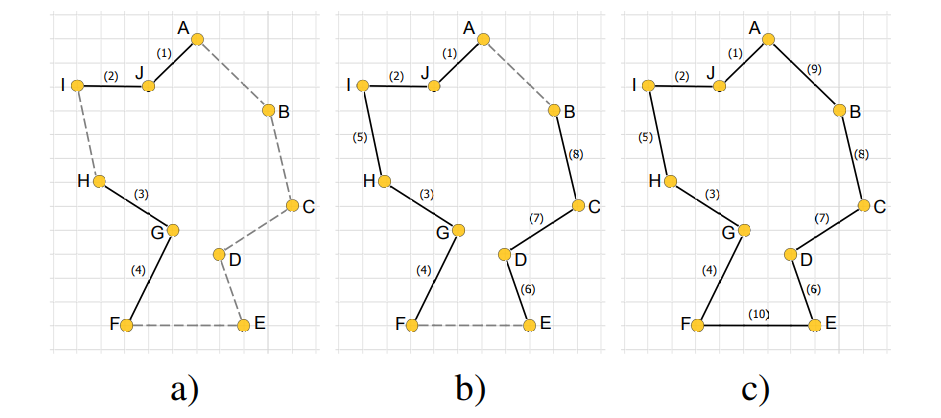
\includegraphics[width=\linewidth]{tspexample.png}
	\caption{Example of the extended nearest neighbor constructive
		procedure (source: \cite{kubalik2014novel})}
	\label{fig:tsp}
\end{figure}


\subsection{Extended Nearest Neighbor Constructive Procedure}
\label{sec:CNNP}
The central objective of the Constructive Nearest Neighbor Procedure (CNNP) is to formulate a valid tour of length \emph{n} based on any given priority list. Note, that the terms ``Extended Nearest Neighbor Constructive Procedure'' and ``Constructive Nearest Neighbor Procedure'' are used interchangibly in this thesis. The procedure begins with \emph{n} separate tour components. Each tour component, denoted as \emph{$ C_k $}, is marked by its boundary cities \emph{$ start_k, end_k $}. Initially, every city serves as its own distinct component, implying \emph{$ start_i = i $} and \emph{$ end_i = i $} for each city \emph{i} from 1 to \emph{n}.

Throughout the procedure, the algorithm iterates over the priority list, using the nearest neighbor heuristic at each step. At each iteration \emph{i}, it processes an element from the priority list \emph{P}[\emph{i}]. Depending on \emph{P}[\emph{i}], a component \emph{$ C_k $} is identified, which may contain one or multiple nodes.

If \emph{P}[\emph{i}] turns out to be a boundary node of \emph{$ C_k $}, the procedure picks the city closest to \emph{P}[\emph{i}] and adds it to the tour. Alternatively, if \emph{P}[\emph{i}] is not a boundary node, it locates the nearest neighbors of the boundary nodes \emph{$ start_k $} and \emph{$ end_k $} of the component \emph{$ C_k $}, labeled as \emph{$ N_1 $} and \emph{$ N_2 $}. Of the two possible edges (\emph{$ N_1, start_k $}) and (\emph{$ N_2, end_k $}), the one with the shorter distance is chosen and added to the tour.

At every step, the process merges two components into a single one. This sequence of actions repeats until only a single component is left, symbolizing the final route.

Figure \ref{fig:tsp} provides a graphical illustration of this procedure, constructing a route from the priority list \emph{P} =\{A, I, H, F, J, E, C, D, G, B\}. As observed, \ref{fig:tsp} a) processes \{A, I, H, F\}, wherein each step selects the shortest link to a node's neighbor, leading to two components \{A, J, I\} and \{F, G, H\}. However, when the node J is considered, it's already part of a component and not a boundary node. Hence, the nearest neighbor is sought from nodes I and A. Since the link between I and H is shorter than that between A and B, the components are connected through the I and H edge. The final route, as shown in \ref{fig:tsp} c), is derived by applying the same rules to the remaining priority list.

As previously mentioned, several priority lists might eventually represent the same route. In this straightforward instance, \{A, I, H, F, J, E, C, D, G, B\}, \{I, C, E, B, H, F, A, J, G, D\}, and \{F, A, C, H, I, E, D, B, G, J\} all lead to the same final route.

\chapter{Proposed method}
This chapter proposes an extended version of the original IREANN algorithm, whose main contribution is the incorporation of a feature extraction and propagation mechanism. This mechanism aims to leverage high-quality features from individual solutions and propagate the knowledge across the entire population. The primary purpose is to increase the algorithm's effectiveness in dealing with complex combinatorial optimization problems. This mechanism is described in detail in section \ref{sec:extension}.

As a test case for the extended IREANN, an arc routing problem named the Capacitated Arc Routing Problem (CARP) was chosen. However, IREANN was originally designed to solve the Travelling Salesman Problem, a vehicle routing problem. That implies some changes to the core IREANN algorithm were necessary to adapt it to the nuances of CARP. CARP introduces additional complexities not present in the Travelling Salesman Problem. It is a more complex problem that not only requires routing, but also involves servicing edges or arcs with specific demands while defining capacity constraints of the vehicles.

The adjustment of the inner representation of routes for each individual in the population and the modification of the nearest neighbor heuristic is crucial for the domain of the CARP, furthermore the adaptation of local search operators specifically for CARP, which play a crucial role in the algorithm's efficiency, is also required.

On the other hand, the core components of the evolutionary framework, specifically, the selection, crossover, and mutation operators remain largely unchanged. This is because these genetic operators are fundamentally problem-independent and can be applied in the same way across a wide variety of combinatorial optimization problems.


\section{CARP Terminology}
It is neccessary to introduce couple terms which are specific to the CARP domain. By the term ``solution'', we refer to the set of routes constructed by the CNNP. A route is a sequence of required edges, and also contains information about between the links between each of the required edges.

route

cumulative cost

number of vehicles


\section{IREANN customizations to CARP}
In CARP, the atomic element shifts from a node to an edge. Instead of cities as it is the case in TSP, the entities to be visited are now the required edges of a graph, each having a specific demand to be serviced. This change in representation has a direct impact on the design of the nearest neighbor heuristic as well, which is a key component in constructing new solutions.

\subsection{Indirect representation}
\label{sec:indirectcarp}
Proposed customized version of IREANN, uses priority list of edges instead of nodes. Similarly to the original IREANN \cite{kubalik2014novel} for TSP, the priority list represents the order in which the nearest neighbor heuristic will be applied, but in this case, on edges during the process of developing the set of tours.

The priority list, serving as the genotype within the evolutionary framework, shifts from representing a sequence of nodes or cities in TSP to representing a sequence of required edges in CARP. The overall functionality remains the same as it was the case in the original version, which means that the priority list represent the order in which the nearest neighbor heuristic is applied.

\subsection{Extended nearest neighbor constructive procedure}
\label{sec:CNNPCARP}
In section \ref{sec:CNNP}, the constructive nearest neighbor procedure (CNNP) was introduced and its functionality was demonstrated on the TSP. However, directly applying the same CNNP to the Capacitated Arc Routing Problem is not as straightforward. The transition to CARP requires several modifications to the CNNP to effectively handle the distinct requirements and constraints of this more complex problem.

Procedure is formally described in Fig. \ref{fig:cnnpcarp}
The process starts with \emph{n} independent tour components, where \emph{n} is the number of required edges. Each required edge initially belongs to its own component. Each component is defined by its boundary nodes {\emph{$start_k$}, \emph{$end_k$}}. A boundary node is a node which belongs to a boundary edge, which is not connected to any other edge via that node. Which means that in the beginning, boundary nodes of all components are the two nodes of each corresponding required edge. 

In each step of the procedure, either two components are merged together if their conjunction satisfies the capacity constraints, or nothing is done if there is no other route that would still meet the constraints after being merged with.

In particular, in \emph{i}-th step the corresponding edge at \emph{i}-th position in the priority list, denoted as working edge \emph{P}[\emph{i}], is taken and the component to which edge \emph{P}[\emph{i}] belongs, \emph{$C_k$}, is identified. As opposed to the original IREANN, this modified version for the CARP is simplified and does care whether the edge \emph{P}[\emph{i}] is boundary edge of \emph{$C_k$}. Nearest available neigbors to the \emph{$start_k$} and \emph{$end_k$} boundary nodes of the component \emph{$C_k$}, \emph{$N_1$} and \emph{$N_2$}, are found. \emph{$N_1$} and \emph{$N_2$} have to meet several conditions which are in place because of the CARP definition. Firstly, both \emph{$N_1$} and \emph{$N_2$} have to be boundary nodes of some other component \emph{$C_j$}, \emph{k} $\neq$ \emph{j}. Such possible candidates have to be filtered out if the sum of demands of required edges in components \emph{$C_k$} and \emph{$C_j$} is greater than \emph{Q}, which would result in a violation of the maximum vehicle capacity constraint \emph{Q}. 

Finally, the shorter path out of (\emph{$N_1$}, \emph{$start_k$}) and (\emph{$N_2$}, \emph{$end_k$}) is added to constructed tour of component \emph{$C_k$}, along with the whole corresponding component \emph{$C_j$} belonging to the selected node (\emph{$N_1$} or \emph{$N_2$}), effectively merging \emph{$C_k$} and \emph{$C_j$} together. A path between two arbitrary nodes, $v_1$ and $v_2$, refers to the shortest possible path on the entire graph $G$. It is important to note that this path can potentially include passing even a required edge. The definition of the CARP permits the passing of required edges without servicing them, allowing for more flexibility in finding the shortest path between the specified nodes.

Note, that it is possible that no other node in the entire graph with its corresponding component satifies the vehicle capacity constraint, which would result in continuing to (\emph{i}+1)-th step right away without extending any component. The procedure ends after all \emph{n} edges from priority list have been processes, at the end, we are left with a certain number of components \emph{$|C|$} $\leq$ \emph{n}, i.e. separate routes each for a single vehicle to take. \emph{$|C|$} might be greater than the maximum number of vehicles allowed \emph{K}, which would make the constructed set of routes an invalid solution, this drawback is discussed in further detail in section \ref{sec:feasibility}.

To sum up the differences between the original constructive procedure for TSP and this modifed version for CARP, most notably we have to check each candidate whether is satisfies the constraint posed by the CARP domain. The rest of the procedure is very similar, we are just dealing with edges instead of individual nodes.



	
\begin{figure}
\begin{algorithmic}[1]
	\State Initialize \emph{n} single edge components \emph{$ start_i = i, end_i = i $} for \emph{$ i = 1, ..., n $}
	\State $j \gets 1$
	\While{$j \leq n$}
	\State Take \emph{j}-th edge, \emph{P}[\emph{j}], from the priority list \emph{P}
	\State Identify component \emph{$ C_k $} to which edge \emph{P}[\emph{j}] belongs
	\State (\emph{$N_1$}, \emph{$C_{N1}$}) $\gets$  {\tt nearestNeighbor}(\emph{$ start_k $}); (\emph{$ C_k $}, \emph{$C_{N1}$}) satisfies \emph{Q} constraint
	\State (\emph{$N_2$}, \emph{$C_{N2}$}) $\gets$  {\tt nearestNeighbor}(\emph{$ end_k $}); (\emph{$ C_k $}, \emph{$C_{N2}$}) satisfies \emph{Q} constraint
	
	\If{{\tt dist}(\emph{$ N_1, start_k $}) $\leq$ {\tt dist}(\emph{$ N_1, end_k $})}
		\State add path(\emph{$ start_k, N_1 $})
		\State merge components(\emph{$C_k, C_{N1}$})
	\Else
		\State add path(\emph{$ end_k, N_2 $})
		\State merge components(\emph{$C_k, C_{N2}$})
	\EndIf
	
	\State \emph{j}++
	\EndWhile
	
	
\end{algorithmic}
	\caption{Extended nearest neighbor constructive procedure modified for CARP}
\label{fig:cnnpcarp}
\end{figure}


 

\subsection{Solution feasibility}
\label{sec:feasibility}
Because of the nature of the capacitated arc routing problem, the challenge of solution feasibility arises. After the evaluation of given individual using the nearest neighbor constructive procedure, it is possible the resulting set of routes violates the constraint of maximum vehicle used. Such problem would not come up if the goal was to solve the Travelling salesman problem using similar heuristic to CNNP, but for the CARP which defines the maximum vehicle contraint, solutions violating this constraint are not acceptable. 

Another constraint is the maximum capacity of each vehicle, meaning that the sum of demands of each required edge in a single route must not exceed the defined limit \emph{Q}, which is same for the whole fleet. The solutions however can not possibly violate this constraint thanks to the way the routes are constructed via the CNNP. (See section \ref{sec:CNNPCARP}) CNNP does not allow a route to be extended with another one which would result in such violation. That results in only the maximum vehicle count constraint being vulnerable to violation, not the maximum capacity one which is always satisfied by the innate design of this approach.

To deal with the infeasibility obstacle, one idea would be to leave every infeasible solution out of the population of candidate solutions and not consider them at all. However, this approach would cause a lot of trouble, because in order to create the initial population, chromosomes of individuals in the first generation are set arbitrarily. Those chromosomes with randomly ordered genes are very unlikely to generate a valid solution in terms of the number of vehicles used, which would make it almost impossible to generate an initial generation of only individuals with feasible solutions.

Instead, individuals representing infeasible solutions are allowed to exist in the population, but we need a way of telling which infeasible solutions are better than others in order to guide the computation in the correct direction and thus converge to a state where there is a population with feasible individuals. 

That is where the fitness evaluation of each individuals comes into play.

\subsection{Individual Fitness}
\label{sec:fitness}
Using the terminology introduced in table \ref{tab:key-concepts}, in the evaluation process the individual's genotype is taken as input. It is then converted to its corresponding phenotype, which serves as the basis for computing the final fitness, which is the output of this procedure.

To make it clear, in the case of our implementation of extended IREANN algorithm for the CARP, genotype is the priority list of required edges, which is what mainly defines each individual. However, because of the indirect representation aspect (see section \ref{sec:indirectcarp}), this priority list (genotype) is converted into the actual set of routes (phenotype) the fleet of vehicle has to travel through via the means of CNNP (see section \ref{fig:cnnpcarp}). It is this set of routes upon which the fitness is computed, not the priority list. Because of the reasons stated in sections \ref{sec:feasibility}, we can not simply define the fitness of an individual by a single number representing the cumulative cost of its set of routes. We also need to capture the count of such set of routes, in order to be able to tell whether the individual violates the maximum vehicle constrained (as discussed in section \ref{sec:feasibility}). 

As a result, the fitness is represented by the pair of values being \emph{$(1)$} the total cumulative cost of the set of routes computed by the CNNP, and \emph{$(2)$} the number of routes in such a set of routes. 

Formally, we define the fitness of an individual as a value pair \{\emph{cost}, \emph{vehicle count}\}, where


Further clarification on why the evaluation of an individual involves a pair of values, rather than just one, is provided in section \ref{sec:feasibility}.


\subsection{Comparison of Individuals}
\label{sec:sorting}
For the reasons stated in section \ref{sec:feasibility}, we have to come up with a mechanism which incentivizes the population to converge to a state where there are only individuals with valid number of vehicles.

Ultimately, the desired functionality is to be able to tell which individuals are the fittest with respect to each other. That enables us to create hierarchy within given population of individuals, giving the more fit individuals higher chance of ``survival'' through the selection operator, which is the main driving force behind the evolutionary process towards finding optimal solutions.

We are not able to establish such a hierarchy just by sorting the population by the measure of the cumulative cost of all the routes in an individual's solution. Although that is the end goal of the whole computation, to find a solution that minimizes this attribute, we can not neglect the number of vehicles used during this process. The reason behind that is the possibility of a situation where a solution with lower cumulative cost and a number of vehicles over the limit \emph{K} would be considered more fit than a solution with satisfactory number of vehicles and a greater cost. Put simply, a solution that violates the constraints defined by CARP (i.e., one with $|\emph{C}| > $ \emph{K}) would be considered more fit than a valid one, which is obviously an undesirable behaviour which would disable the evolutionary process from achieving any progress.

Optimization of two variables at the same time is not possible, so the fitness evaluation will prioritize driving the vehicle count down first, and after that optimize the total routes cost when a satisfactory vehicle count has been reached.
This desired functionality is achieved by designing a custom comparator, that decides which one of two individuals is "more" fit. This comparator is utilized to sort the population, which results in having an ordered sequence of individuals with the fittest ones at the beginning. In the end, that is what the fitness function is for, to tell how good the solutions are with respect to each other so that during the selection phase (details in section \ref{sec:selectioncarp}), the right individuals in population are picked to be mated with each other, according to the selection rules. 

Comparator is a method which takes two individuals as input and decides which one of them is more fit according to criteria mentioned above. Several options might occur:
\begin{itemize}
	\item Vehicle count of both individuals is greater than the limit, then the one with lower vehicle count is deemed more fit. The cost is the deciding factor only when the vehicle counts are equal.
	\item First individual has satisfactory vehicle count, the other has not. In this case, the first individual is preferred no matter the cost of their solution.
	\item Both vehicle counts are less or equal than the limit, then the individual with lower cost is preferred.
\end{itemize}

\subsection{Selection}
\label{sec:selectioncarp}
It is through effective selection that promising individuals are identified and retained, contributing to the improvement of solutions over time. It is the iterative process of selecting and evaluating individuals which guides the evolutionary algorithm towards better performing solutions.

In our implementation, the tournament selection method is utilized as the primary selection mechanism. This method involves selecting a fixed number of individuals, known as the tournament size, from the population. The tournament size is an arbitrary hyperparameter that can be adjusted based on the desired selection pressure. The individual with the best fitness score is the winner of that tournament.

By choosing a larger tournament size, more individuals participate in each tournament, increasing the competition and favoring the selection of fitter individuals. This intensifies the selection pressure and promotes exploitation of promising solutions. Conversely, a smaller tournament size allows weaker individuals to have a better chance of being selected, facilitating exploration and diversifying the population.

In our case, we need to run the tournament selection twice in order to obtain the parent individuals needed to produce an offspring. Our tournament selection procedure has two paramenters \emph{$t_1$} and \emph{$t_2$}, which represent the tournament sizes for both selected parents. Both group of individuals in each tournament are sorted according to our comparator described in section \ref{sec:fitnesscarp}, and the first element, considered the winner of a tournament is selected to be one of the parents for the offspring, which is about to generated through means of recombination from the two parent individuals.

\subsection{Crossover}
After performing the tournament selection process on the current population, a pair of parent individuals is selected. For each pair of parents, two offspring are created using crossover and mutation operators. 

We used an \emph{order-based crossover}, defined by Syswerda in \cite{syswerda1991schedule}. The crossover constructs an offspring so that first several cities randomly chosen from the priority list of the first parent are copied to the offspring into the same positions as they appear in the parent. The remaining positions are filled in with the remaining cities, in the same relative order as in the second parent.

\subsection{Mutation}
Mutation operator is very simple, it randomly changes the position of a single edge in the priority list. While some argue that memetic algorithms may not require a mutation operator due to the local search component, we have chosen to retain it in our algorithm. The mutation operator provides an additional source of exploration and helps maintain genetic diversity within the population.

\subsection{Local search optimization}
\label{sec:localsearchcarp}
Local search procedures, introduced in \ref{sec:localsearch} play a crucial role in yielding competitive results.

We implemented several local search procedures, which operate on the phenotype level of solutions. That means, we try to tweak the inner solution representation ever so slightly (i.e., modify the set of routes in one of many ways), while seeking improvement in the objective function. If we come across such an improvement, we incorporate it into the representation of given individual.

Our implementation of local search operators was heavily inspired by the work \cite{tang2009memetic} by Tang, Mei and Yao. They presented one of the most famous algorithms for solving the capacitated arc routing problem, abbreviated the "MAENS". Several local search heuristics utilized in MAENS were in some form adopted for this implementation.

Firstly, we list three traditional move operators, namely the single insertion, reversal and 2-opt moves. All of the moves mentioned operate in a deterministic manner, trying out every possible combination looking for improvement in the fitness score. A greedy approach is favored, which means that if an improvement is found, it is applied right away.

\subsubsection{Single insertion}
In single insert move, an edge is removed from its current position and reinserted into another position in the sequence of edges. Edge might be reinserted either to the route, in which it originally was, or to any other route is the whole set that given individual possesses.

\subsubsection{Reversal moves}
Reversal move simply reverses the direction of an edge. 

\subsubsection{2-opt moves}
We differentiate between two types of 2-opt moves, one for a single route and the other for double routes.
2-opt for single route reverses the direction of its whole subroute, and reconnects it accordingly.
2-opt for double routes disconnects two routes, which results in four different subroutes, which are then optimally reconnected.


\subsubsection{Merge-Split operator}
As the authors of \cite{tang2009memetic} argue, all of the traditional move operators mentioned above adopt a rather simple schemes to generate new solutions, which results in new solutions that are very similar to the original ones. They describe them as having a "small" step size, thus being capable of searching only a "small" neighborhood.
It is further discussed, that it would be neat to have a move operator with larger step size. That could be theoretically achieved by extending the traditional move operators, but would be too computationally demanding. For that purpose, the Merge-Split (MS) operator is devised by the authors of \cite{tang2009memetic}.

Our implementation takes inspiration from MS operator and uses a simplified version, the improvements it yields are vastly superior to traditional move operators.
It basically selects \emph{p}(\emph{p}>1) routes of a given individual, merges them together and tries to reconnect them in a way that leads to a decrease in the total cost. When reconnecting this subset of individual's set of routes, the same constructive procedure to the one used during evaluation of offsprings is employed. Which basically means, that we are trying to reconnect all the edges in the selected subset again via the CNNP, but this time, all the edges which are part of routes that were not selected by the MS operator, are not visible at all. That heavily influences the workings of CNNP, which thanks to this functionality is very likely to discover new possible connections, which would be unattainable if the CNNP considered every single edge in the graph as it is the case during standard offspring evaluation. 


\subsection{Dealing with duplicate solutions}
\label{sec:duplicates}
Maintaining a diverse population is crucial in evolutionary algorithms to ensure effective exploration of the search space and avoid premature convergence to suboptimal solutions. One aspect of diversity is the absence of duplicate individuals within the population. Duplicates can limit the exploration capability of the algorithm by occupying multiple slots with identical solutions, reducing the diversity of available genetic material. By preventing duplicates, the algorithm is encouraged to explore a wider range of solutions, increasing the chances of finding better and more diverse solutions. Additionally, a diverse population facilitates the exploration of different regions of the search space, enhancing the algorithm's ability to converge to high-quality solutions.

It would be easy to ensure that there are no two individuals with the same genotype, i.e. priority list. But if two individuals have exactly the same priority lists, they might still be different on the phenotype level. Their inner representation might differ thanks to the local search procedures applied. That is why we came up with a way of checking for duplicity on a deeper level, where the inner representation of each individual is considered. Basically, two individuals are deemed identical, if the set of routes each of them possesses, is exactly the same.

There still may be cases where allowing a certain degree of duplicity can be advantageous. To address this, we introduce a parameter called \emph{maxDuplicates}, which specifies the maximum number of identical individuals with the same set of routes that are allowed to proceed to the next generation. This parameter offers a level of control over the tolerance for duplicity within the population. The effects of this tweaking this paramaters are demonstrates in experimental study chapter of this thesis.

\begin{figure}
	\begin{algorithmic}[1]
		\State population $\gets$ createInitialPopulation()
		\State \emph{j} $\gets$ 0
		\For{$i = 0$ to $maxGenerations$}
		
		\If{$i \geq$ \emph{M} $\land$ \emph{j} \% \emph{k} == 0}
		\State guten tag
		\EndIf
		
		
		\State $\text{interPop} \gets \text{empty list}$
		\State $\text{interPopSize} \gets 0$
		\While{$\text{interPopSize} < \text{popSize}$}
		\State $\text{parent1} \gets \text{tournamentSelection}(\text{population})$
		\State $\text{parent2} \gets \text{tournamentSelection}(\text{population})$
		
		\If{$\text{random.nextDouble()} < \text{probCross}$}
		\State $\text{child1} \gets \text{parent1.crossover(parent2)}$
		\State $\text{child2} \gets \text{parent2.crossover(parent1)}$
		\If{$\text{random.nextDouble()} < \text{probMutation}$}
		\State $\text{child1.mutate()}$
		\State $\text{child2.mutate()}$
		\EndIf
		\Else
		\State $\text{child1} \gets \text{parent1.mutate()}$
		\State $\text{child2} \gets \text{parent2.mutate()}$
		\EndIf
		
		\State $\text{child1.evaluate()}$
		\State $\text{child2.evaluate()}$
		
		\State $\text{child1.localOptimisation()}$
		\State $\text{child2.localOptimisation()}$
		
		\State $\text{interPop.add(child1, child2)}$
		\State $\text{interPopSize} \gets \text{interPopSize} + 2$
		\EndWhile
		\State population = population $\cup$ interPop
		\State $\text{population = sortPopulation(population)}$
		
		\State $\text{population} \gets \text{deleteDuplicates(population)}$
		\EndFor
		
		
		
	\end{algorithmic}
	\caption{Pseudocode of the Extended IREANN}
	\label{fig:evoalg}
	
\end{figure}

\subsection{Extended IREANN algorithm}
\label{sec:evolution}
All the components discussed in this chapter are combined to form an extended IREANN algorithm, which addresses the capacitated arc routing problem. The proposed algorithm falls under the category of memetic algorithms and builds upon the IREANN algorithm \cite{kubalik2014novel}, incorporating modifications specific to the CARP, as well as a mechanism, which during computation identifies high-quality features and propagates that information across the entire population (described in detail in chapter \ref{sec:extension}).

Figure \ref{fig:evoalg} gives an overview of the extended IREANN in pseudocode. As we can see, the computation consists of \emph{maxGenerations} number of total generations. Firstly, an initial population of candidate solutions is created by means of random perturbation of a list of all required edges. All of these individuals in the initial population are expected to be a very poor quality.

During each iteration of the evolutionary process, a new population of offspring individuals, referred to as the "interPopulation," is created. This interPopulation is the same size as the original population. Depending on the value of parameters \emph{probCross} and \emph{probMutation}, a different way of generating an offspring might be employed. \emph{probCross} represent the probability, that offsprings will be, in given iteration, generated via the means of crossover operator. \emph{ProbMutation} represents the probability those offspring are further mutated to achieve more genetic variety. With probability $1 -$ \emph{probCross}, the offspring in that single generation will have the same priority lists as their parent, except they are just mutated. It is reasonable to keep the value of parameter \emph{probCross} close to 1.

The fitness of each new offspring created in the interPopulation is then evaluated through a process described in section \ref{sec:fitness}. This fitness score is then further improved by numerous local search procedures introduced in \ref{sec:localsearchcarp}.

The two populations are then merged into a single one, which is twice the size. This large population is then sorted according to criteria described in section \ref{sec:sorting}, favoring the "more fit" individuals to be listed closer to the beginning of this sequence. Only the first half this sorted large population survives and ``makes it'' to the next generation (becoming the new resulting population the same size as in the beginning of this process), the second half of individuals is considered to be of lesser a quality and is tossed away. A mechanism that filteres out duplicate candidates, i.e. identical individuals is incorporated as well, explanation is provided in section \ref{sec:duplicates}.


\section{IREANN extensions}
\label{sec:extension}
As a primary contribution of this thesis, we have proposed an enhancement to the IREANN algorithm, specifically adapted for the capacitated arc routing problem (CARP). The key driving force behind this extension is the potential of local search operators to make substantial improvements and the existing algorithm's lack of a mechanism to share these valuable insights throughout the entire population. As it stands, each time a new offspring is evaluated, which implies the construction of a new set of routes through the Constructive Nearest Neighbor Procedure (CNNP), the process does so without the advantage of any prior knowledge or insight.

The extension we introduce incorporates a process we've named ``analysis.'' This mechanism periodically computes and retains data regarding the characteristics contributing to high-quality solutions. This stored information is then incorporated into the CNNP, acting as an intermediary to the actual distance information between two nodes. In essence, this extension enriches the algorithm's knowledge pool, enabling it to construct better solutions by utilizing insights from previous successful configurations.





\chapter{Experiments}




\bibliographystyle{amsalpha}
\bibliography{references}


\end{document}